%%%%%%%%%%%%%%%%%%%%%%%%%%%%%%%%%%%%%%%%%%%%%%%%%%%%%%%%%%%%%%%%%%%%%%
% writeLaTeX Example: Academic Paper Template
%
% Source: http://www.writelatex.com
%
% Feel free to distribute this example, but please keep the referral
% to writelatex.com
%
%%%%%%%%%%%%%%%%%%%%%%%%%%%%%%%%%%%%%%%%%%%%%%%%%%%%%%%%%%%%%%%%%%%%%%
% How to use writeLaTeX:
%
% You edit the source code here on the left, and the preview on the
% right shows you the result within a few seconds.
%
% Bookmark this page and share the URL with your co-authors. They can
% edit at the same time!
%
% You can upload figures, bibliographies, custom classes and
% styles using the files menu.
%
% If you're new to LaTeX, the wikibook is a great place to start:
% http://en.wikibooks.org/wiki/LaTeX
%
%%%%%%%%%%%%%%%%%%%%%%%%%%%%%%%%%%%%%%%%%%%%%%%%%%%%%%%%%%%%%%%%%%%%%%
\documentclass[twocolumn,showpacs,%
  nofootinbib,aps,%superscriptaddress,
  eqsecnum,prd,notitlepage,showkeys,10pt]{revtex4-1}
  
\usepackage{amssymb}
\usepackage{amsmath}
\usepackage{graphicx}
\usepackage{dcolumn}
\usepackage{threeparttable}
\usepackage{algorithm}
\usepackage{algpseudocode}
\usepackage[hidelinks]{hyperref}
\usepackage[T1]{fontenc}
\usepackage{array}
\usepackage{makecell}
\newcolumntype{x}[1]{>{\centering\arraybackslash}p{#1}}
\usepackage{tikz}
\usepackage{pgfplots}

% table thick line
\makeatletter
\newcommand{\thickhline}{%
    \noalign {\ifnum 0=`}\fi \hrule height 1pt
    \futurelet \reserved@a \@xhline
}

\newcommand\diag[4]{%
  \multicolumn{1}{p{#2}|}{\hskip-\tabcolsep
  $\vcenter{\begin{tikzpicture}[baseline=0,anchor=south west,inner sep=#1]
  \path[use as bounding box] (0,0) rectangle (#2+2\tabcolsep,\baselineskip);
  \node[minimum width={#2+2\tabcolsep-\pgflinewidth},
        minimum  height=\baselineskip+\extrarowheight-\pgflinewidth] (box) {};
  \draw[line cap=round] (box.north west) -- (box.south east);
  \node[anchor=south west] at (box.south west) {#3};
  \node[anchor=north east] at (box.north east) {#4};
 \end{tikzpicture}}$\hskip-\tabcolsep}}


\begin{document}

\title{Practical Application of Keystroke Dynamics Authentication}

\author{Yuankai Guo}
\email{u0942867@utah.edu}
\affiliation{University of Utah}
\author{Myungho Jung}
\email{myungho.jung@utah.edu}
\affiliation{University of Utah}
\author{Junwei Shi}
\email{sjwarthas2009@gmail.com}
\affiliation{University of Utah}
\author{Xu Wang}
\email{xu724@cs.utah.edu}
\affiliation{University of Utah}

%\begin{abstract}
%Keystroke dynamics has been studied for many years and proved that each user's keystroke pattern is unique. Through the project, we developed a login application to authenticate users by comparing keystroke patterns. We also %tested possible variation of patterns on controlled environment. Unlike other studies, we considered how to apply the mechanism to existing web services.
%\end{abstract}

\maketitle

\section{Introduction}
Password authentication has been one of the most popular method to identify. It is ubiquitous for systems such as Web sites, SSH, and mobile phones. However, attackers' techniques to steal password have also been developed in many ways. Therefore, we need to collect additional information to figure out identity other than just plain text of passwords. For example, access from different IP or MAC address can be suspected as an attack. However, it makes users inconvenient if they are travelling or buy a new device. Keystroke dynamics can be extracted while typing password as well as used as identity verification\cite{gaines1980authentication}. The existing users don't have to buy an additional device. Only a small change in the server will be required to apply this mechanism.

\section{Related Works}
Many algorithms to detect outliers were studied and test on performance and precision\cite{shanmugapriya2009survey}. The various algorithms were used for pattern matching, such as neural network, Support Vector Machines, K-Nearest Neighbors, and Euclidean distance. For most researches, hundreds of patterns from dozens of people were collected and tested. Unlike those studies which tested on practical experiments, we focused on the variation of the users. One of the defects of the result from most existing tests is that they intentionally collected data from people in a short period of time. If the group only consists of experienced users, the data would be biased. Also, the variation of patterns cannot be observed in a short period of data. In some cases, a test in well-controlled environment can produce more reliable result than practical experiments.

\section{Threat Model}
Password-based authentication is ubiquitous for identification on the internet. However, as the number of web services has dramatically increased, it becomes impossible for people to remember tons of passwords and most of them are using the same password for all web sites. It will be a problem if a cracker breaks in a insecure server and steals users' passwords, the password can be used for other web services as well. Therefore, it will be useless even if a web site is protected by almost perfect secure system.\par
Unlike the password, keystroke dynamics is one of the biometric authentication such as face, fingerprint, and iris recognition\cite{karnan2011biometric}. Thus, it changes as time goes as well as it can be stored as a data structure which is appropriate to compare similarity but it is difficult to imitate the pattern. Also, the method can be applied on the existing password authentication system as an additional layer. It will make the authentication system more secure and robust.

\section{Method}
\subsection{Data structure}
\begin{figure}[h]
  \centering
  \includegraphics[width=0.5\textwidth]{keystroke}
  \caption{Timing measurement in interval and duration}
  \label{fig:keystroke}
\end{figure}

The timing vector of keystroke patterns can be measured as intervals between keys and keystroke durations\cite{cho2000web}. Therefore, a pattern of $n+1$ numbers will be created from typing $n$ characters password including return key. In most studies, the vector is measure like this; however, as seen in Figure \ref{fig:keystroke}, we applied it in a slightly different way. The interval in our project measured not from previous release time but from previous press time. By doing so, there is no negative value and storage can be saved by store only unsigned data. The timing vector can be considered as a point in $n+1$ dimensional space. Then, we can measure the distance of two points, and apply machine learning or neuron network algorithm to detect novelties.
\par
The pattern needs to be normalized because the storage is limited and in order to equivalent comparison among users. First, the timing values are divided by the maximum value and stored with the maximum value. Then, the values becomes less than 1 and the data size can be controlled by floating point precision. Also, two different length of passwords cannot be evaluated with the same error bound. Therefore, the sum of values should be divided by a factor of dimension of the point. Or if the computation is not obvious, we can multiply the error bound by $\sqrt{d}$ such that $d$ is the order of dimension.

\section{Algorithm}
\subsection{Novelty Detection}
To filter imposter's patterns, a novelty detection algorithm is required. There are many researches to detect anomaly. The algorithms can be divided into statistical type, neural network, pattern recognition based on learning, and heuristics\cite{banerjee2012biometric}. We tested three common algorithms, which are the Nearest Neighbor, Mahalanobis distance, and one class SVMs, with changing the patterns.

\section{Implementation}

\section{Analysis}
The performance of statistical and machine learning algorithms have already been tested in many studies. Thus, we focused on expecting actual users' patterns. Previous works are based on heuristic results or similar dataset. However, the pattern may not be even even if the same person types several times. It would be came from using different type of input devices or physical changes. For instance, it will show different patterns when using PC and keyboard than using mobile devices. Also, the more familiar users become to type the same password, the faster they type. Therefore, we tried to form as reliable synthetic environment as possible for the test. We tested the environment with assumptions and measured error rates. The error rates for pattern detection are divided into two parts which are False Acceptance Rate(FAR) and False Rejection Rate(FRR)\cite{cho2000web}. For each test case, the two error rates are computed for comparing performance.

\subsection{Environment}
Test program is coded in python using Scipy, Numpy, and scikit-learn library. For each test, 1000 evenly distributed patterns of imposters are generated because we want to simulate the environment that a lot of imposters try to imitate the pattern. Also, the same number of patterns of genuine users are generated with satisfying gaussian distribution. It would be similar to a user's patterns. Unlike other researches, we tried to predict the variation of patterns.\par
Our tests are focused on the variation of the patterns over time. First, only an interval of patterns would be different each time. Suppose that the password is mixed with a sequence of alphabets and that of numbers like `abcd1234.' In this cases, the user's patterns between word and numbers may not be expected. Second, we assume that the user's patterns would be fast or slow; however, those will be proportional. The ratio of keystroke pattern of a user will not change much even if the speed is different depending on the condition. Finally, the user may use different types of keyboards such as portable keyboard or touch keyboard on mobile devices other than regular keyboard. Then, we expect the patterns would form multiple clusters.

\subsubsection{Test Results}
\begin{figure}[ht]
  \centering
  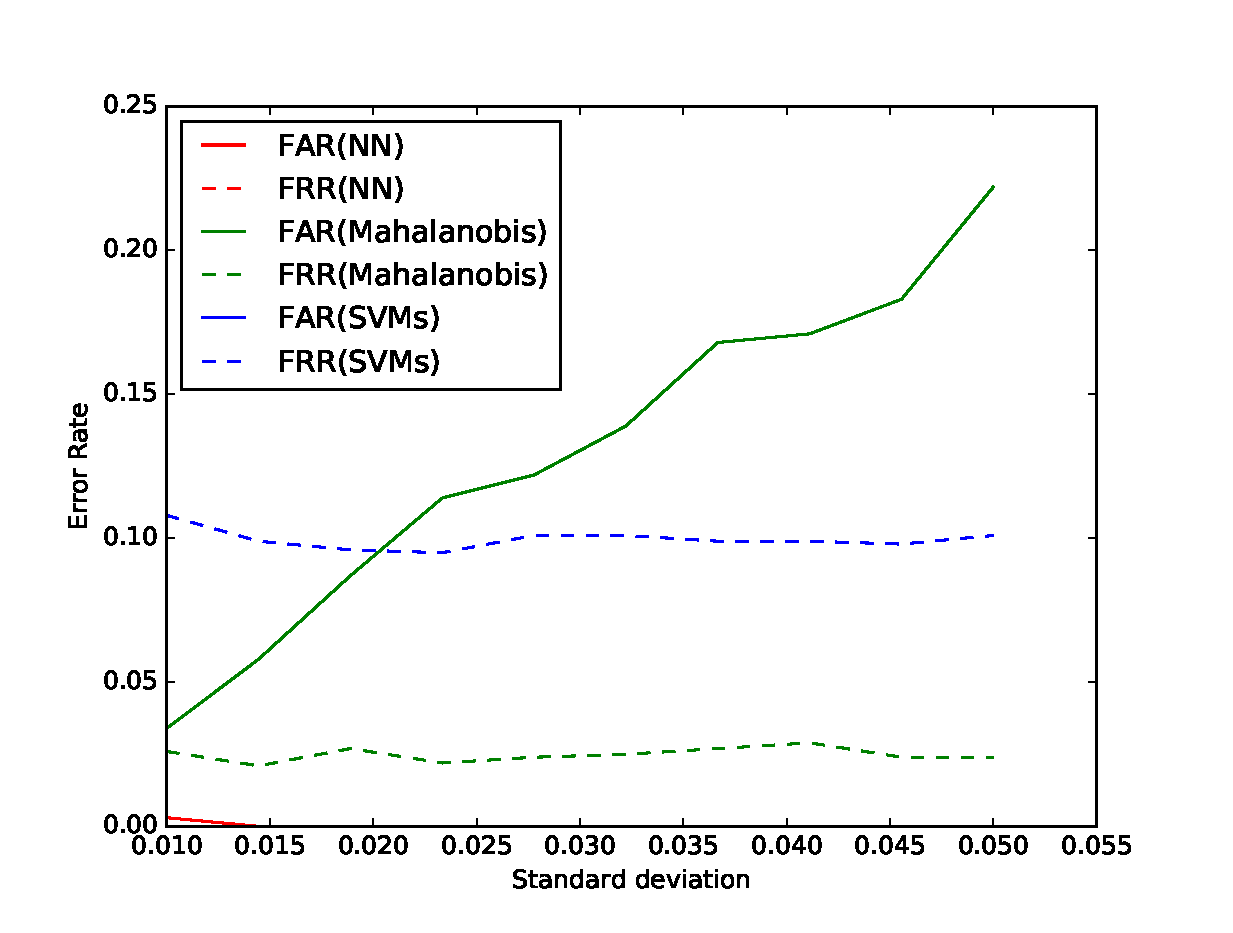
\includegraphics[width=0.5\textwidth]{one}
  \caption{Test result of patterns that only one of the intervals varies}
  \label{fig:one}
\end{figure}
\begin{figure}[ht]
  \centering
  \includegraphics[width=0.5\textwidth]{prop}
  \caption{Test result of proportional patterns}
  \label{fig:prop}
\end{figure}
\begin{figure}[ht]
  \centering
  \includegraphics[width=0.5\textwidth]{multi}
  \caption{Test result of patterns of multiple clusters}
  \label{fig:multi}
\end{figure}

Most of the error rates are not visible because they are very close to 0. As seen in the three tests, we concluded that the performances of the three algorithms are not much different regardless of the variation of the patterns. The most accurate method among them was the nearest neighbor method, the SVMs was next, and the Mahalanobis distance showed the worst performance. And with respect to computation time, the SVMs was the fastest, the nearest neighbor was next, and the Mahalanobis distance was the slowest. However, it would be the difference in library used. The SVMs and nearest neighbor using ball tree was implemented using scikit-learn library. On the other hand the Mahalanobis distance was measured using scipy library.

\section{Defects}
Although there are many researches and practical application of Keyboard Dynamics, there are problems in authenticating with the method. Assume that the mechanism is applied for Web-based system. Then, people can move cursors using arrow keys or mouse while typing and editing password. We just ignored the cases and assumed that the web page allows only password typed at once. Though it would make the users inconvenient, the web service will become more secure. If the mechanism is used for SSH, we don't have to worry about problems caused by arrow keys and mouse. However, there is still problems on pressing backspace key. For security enhancement, it is necessary to block the key inputs and use of mouse on the password window.\par
Also, it is possible to sneak key timing patterns by spyware with key logger. Even if the pattern is encrypted before sent, the attacker can sneak the patterns recorded by the key logger. This type of threat can be prevented by sharing a nonce with server. This is the process: add the nonce to the key pattern, encrypt the pattern, send it to server, and the server decrypts and subtract the shared nonce. By doing so, even if the attacker stole the pattern, it would not match with the users pattern.\par
In addition, a user's patterns change more frequently than other physiological traits or behavioral characteristics. We suggested a system that evaluates only the latest patterns like sliding window.

\section{Conclusion}
Through the project, we checked the algorithm is working by demo program and also tested the performance between algorithms. We suggested that the possible web-based authentication using keystroke dynamics by implementing and testing actual login web page. Unfortunately, it is not sure that the test data is significant compared to that from other research. However, the application developed for the experiments will be useful to test other algorithms with a myriad of possible fixed patterns and variations. It will help to create various environments for experiments.

%%%%%%%%%% BIBLIOGRAPHY %%%%%%%%%%
\bibliographystyle{plain}
\bibliography{report}

\end{document} 